\documentclass[border=4pt]{standalone}
% shared style for all PyTBA topology diagrams (\input by each standalone file)
\usepackage{mathpazo}
\usepackage{amsmath}
\usepackage{tikz}
\usetikzlibrary{positioning,arrows.meta,calc,decorations.pathreplacing,fit,backgrounds}
\tikzset{
  host/.style={draw=blue!55!black, fill=blue!7, rounded corners=2pt, align=center,
               minimum height=9mm, minimum width=22mm, font=\small},
  blk/.style={draw=black!60, fill=black!4, rounded corners=2pt, align=center,
              minimum height=8mm, font=\small},
  chan/.style={draw=orange!70!black, fill=orange!8, rounded corners=2pt, align=center,
               minimum height=9mm, font=\small},
  lossbox/.style={draw=red!70!black, fill=red!6, rounded corners=2pt, align=center, font=\footnotesize},
  data/.style={-{Stealth[length=2.2mm]}, thick},
  ack/.style={-{Stealth[length=2mm]}, dashed, black!60},
  lbl/.style={font=\footnotesize, align=center},
  brace/.style={decorate, decoration={brace, amplitude=4pt}, thick, black!70},
}

\begin{document}
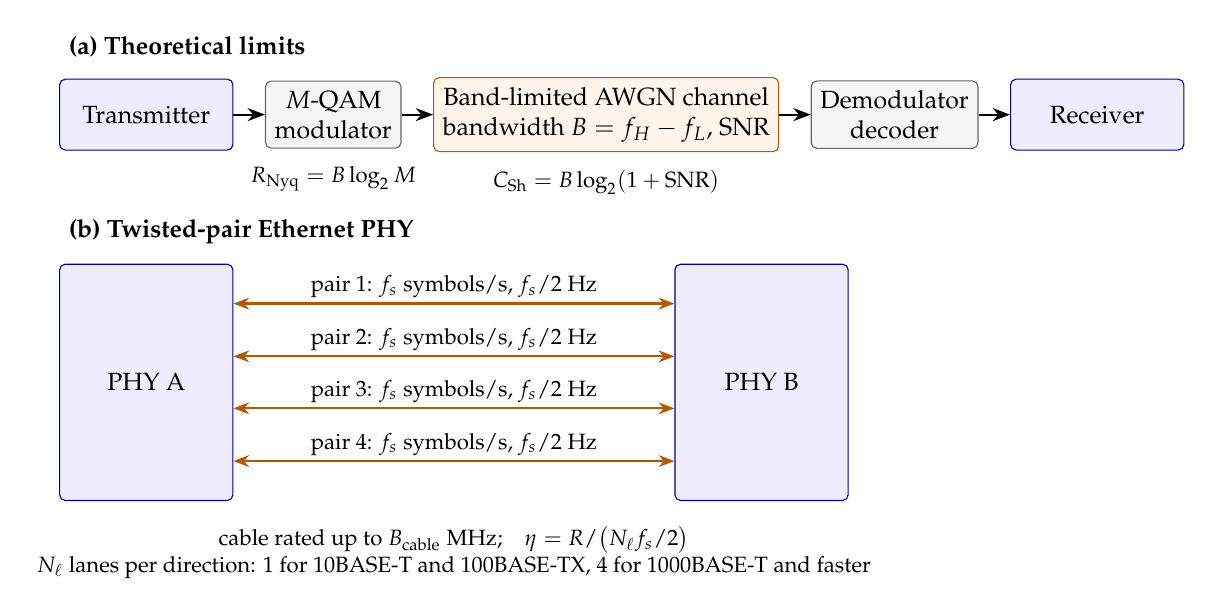
\begin{tikzpicture}[node distance=4mm]
% (a) generic band-limited channel
\node[host] (tx) {Transmitter};
\node[blk, right=of tx] (mod) {$M$-QAM\\modulator};
\node[chan, right=of mod, minimum width=30mm] (ch) {Band-limited AWGN channel\\bandwidth $B=f_H-f_L$, SNR};
\node[blk, right=of ch] (dem) {Demodulator\\decoder};
\node[host, right=of dem] (rx) {Receiver};
\draw[data] (tx) -- (mod); \draw[data] (mod) -- (ch); \draw[data] (ch) -- (dem); \draw[data] (dem) -- (rx);
\node[lbl, below=1mm of mod] {$R_{\mathrm{Nyq}}=B\log_2 M$};
\node[lbl, below=1mm of ch] {$C_{\mathrm{Sh}}=B\log_2(1+\mathrm{SNR})$};
\node[font=\small\bfseries, anchor=west] at ($(tx.north west)+(0,4mm)$) {(a) Theoretical limits};
% (b) twisted-pair Ethernet PHY
\begin{scope}[yshift=-34mm]
\node[host, minimum height=30mm] (pa) {PHY A};
\node[host, minimum height=30mm, right=56mm of pa] (pb) {PHY B};
\foreach \i/\y in {1/10,2/3.3,3/-3.3,4/-10} {
  \draw[{Stealth[length=2mm]}-{Stealth[length=2mm]}, thick, orange!70!black]
     ($(pa.east)+(0,\y mm)$) -- node[lbl, above=-0.6mm, black] {pair \i: $f_s$ symbols/s, $f_s/2$ Hz}
     ($(pb.west)+(0,\y mm)$);
}
\node[lbl, below=2mm of $(pa.south)!0.5!(pb.south)$] {cable rated up to $B_{\mathrm{cable}}$ MHz;\quad $\eta = R/\big(N_\ell f_s/2\big)$\\
   $N_\ell$ lanes per direction: 1 for 10BASE-T and 100BASE-TX, 4 for 1000BASE-T and faster};
\node[font=\small\bfseries, anchor=west] at ($(pa.north west)+(0,4mm)$) {(b) Twisted-pair Ethernet PHY};
\end{scope}
\end{tikzpicture}
\end{document}
